\documentclass[11pt, oneside]{article}   	% use "amsart" instead of "article" for AMSLaTeX format
\usepackage{geometry}                		% See geometry.pdf to learn the layout options. There are lots.
\geometry{letterpaper}                   		% ... or a4paper or a5paper or ... 
%\geometry{landscape}                		% Activate for for rotated page geometry
%\usepackage[parfill]{parskip}    		% Activate to begin paragraphs with an empty line rather than an indent
\usepackage{graphicx}				% Use pdf, png, jpg, or eps§ with pdflatex; use eps in DVI mode
								% TeX will automatically convert eps --> pdf in pdflatex		
\usepackage{amssymb}
\usepackage{amsmath}

\usepackage{tikz} % Flow charts
\usetikzlibrary{shapes,arrows}
\usetikzlibrary{trees}

\tikzstyle{decision} = [diamond, draw, fill=blue!20, text width=4.5em, text badly centered, node distance=3cm, inner sep=0pt]
\tikzstyle{block} = [rectangle, draw, fill=blue!20, text width=3cm, text centered, rounded corners, minimum height=4em]
\tikzstyle{line} = [draw, -latex', text width=3cm]
\tikzstyle{cloud} = [draw, ellipse,fill=red!20, node distance=3cm, minimum height=2em]

% Set the overall layout of the tree
\tikzstyle{level 1}=[level distance=5.3cm, sibling distance=2cm]
\tikzstyle{level 2}=[level distance=5.3cm, sibling distance=2cm]

% Define styles for bags and leafs
\tikzstyle{bag} = [text width=0.6cm, text centered]
\tikzstyle{bag2} = [text width=3.5cm, text centered]
\tikzstyle{end} = [circle, minimum width=3pt,fill, inner sep=0pt]

\title{Pandora Analysis Calibration Binaries Explained}
\author{Steve Green}
\date{}							% Activate to display a given date or no date

\begin{document}
\maketitle

%------------------------------------------------
% Abstract
%------------------------------------------------

\begin{abstract}
An introduction into the calibration procedure required for simulation of events at a future linear collider using the particle flow algorithm PandoraPFA is described in full.  The calibration procedure covers the setting of constants used at both the digitisation stage of reconstruction as well as the calibration constants used within PandoraPFA.  Recalibration must be performed for all changes to detector design and/or particle reconstruction in PandoraPFA.
\end{abstract}

%------------------------------------------------
% Introduction
%------------------------------------------------

\section{Introduction}

The following process sets a series of constants related to the digitisation stage (Table \ref{table1}) and in the particle reconstruction within PandoraPFA (Table \ref{table2}).

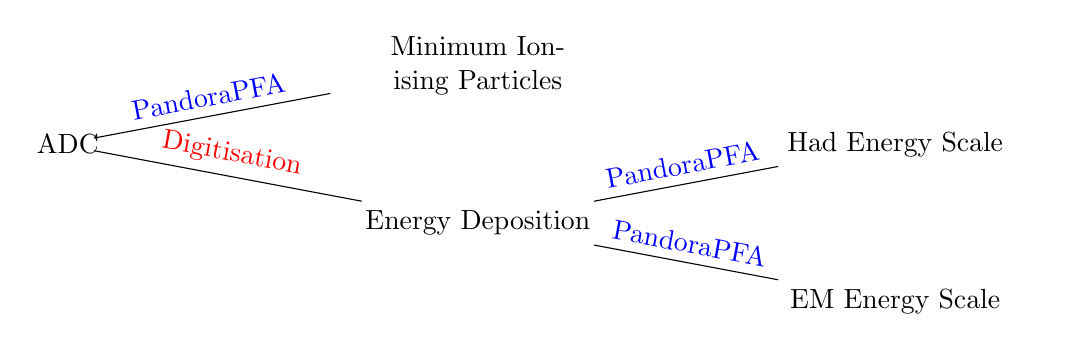
\begin{tikzpicture}[grow=right, sloped]
Overview of constants set in this procedure:
\node[bag] {ADC}
    child {
        node[bag2] {Energy Deposition}        
            child {
                node[bag2, label=right:{}] {EM Energy Scale}
                edge from parent
                node[above] {\textcolor{blue}{PandoraPFA}}
            }
            child {
                node[bag2, label=right:{}] {Had Energy Scale}
                edge from parent
                node[above] {\textcolor{blue}{PandoraPFA}}
            }
            edge from parent 
            node[above] {\textcolor{red}{Digitisation}}
    }
    child {
        node[bag2, label=right:{}] {Minimum Ionising Particles}   
            edge from parent
            node[above] {\textcolor{blue}{PandoraPFA}}
    };
\end{tikzpicture}

\begin{table}[htdp]
\caption{Digitisation Constants}
\begin{center}
\begin{tabular}{|c|l|}
\hline
Constant & Description \\
\hline
CalibrECAL 		& Converts the ADC current to an energy deposition in units of \\
                    		& GeV in the ECal \\
CalibrHCALBarrel 	& Converts the ADC current to an energy deposition in units of \\
                    		& GeV in the HCal Barrel \\
CalibrHCALEndcap 	& Converts the ADC current to an energy deposition in units of \\
                   		& GeV in the HCal Endcap\\
CalibrHCALOther 	& Converts the ADC current to an energy deposition in units of \\
                    		& GeV in the HCal Other (i.e. Ring) \\
\hline
\end{tabular}
\end{center}
\label{table1}
\end{table}%

\begin{table}[htdp]
\caption{PandoraPFA Constants}
\begin{center}
\begin{tabular}{|c|l|}
\hline
Constant & Description \\
\hline
ECalGeVToMIP 			& Converts ADC measurements to units of number of\\
			 			& MIPs in the ECal\\
HCalGeVToMIP 			& Converts ADC measurements to units of number of\\
			 			& MIPs in the HCal\\
MuonGeVToMIP 			& Converts ADC measurements to units of number of\\
			 			& MIPs in the Muon Chamber\\
ECalToEMGeVCalibration 	& Energy rescaling factor for electromagnetic energy\\
					 	& in the ECal \\
HCalToEMGeVCalibration 	& Energy rescaling factor for electromagnetic energy\\
					 	& in the HCal \\
ECalToHadGeVCalibration 	& Energy rescaling factor for hadronic energyl\\
					 	& in the ECal \\
HCalToHadGeVCalibration 	& Energy rescaling factor for hadronic energy\\
					 	& in the HCal \\
\hline
\end{tabular}
\end{center}
\label{table2}
\end{table}%

A series of executable files have been produced to determine the values that each of these calibration constants can take.  These executables can be found within the calibration folder inside the PandoraAnalysis package. A description on how to use each of these executables follows.  It should be noted that the setting of these calibration constants is an iterative process.

\section{Calibration Files}

Each of these executables takes in a series of single particle root files, which must have been produced from a recent version of Pandora Analysis (revision 1668 or later).  To perform the full calibration procedure a series of PfoAnalysis trees are needed that have been produced from the simulation of single particle events using the detector model being examined.  The PfoAnalysis trees are generated from the PfoAnalysis processor, which is found in PandoraAnalysis.  

To collect the relevant calibration information within the PfoAnalysis processor a series of extra parameters must be specified in the xml steering file.  These include the sim calo hit collections produced from GEANT (via Mokka) and the calorimeter hit collections produced from the digitisation stage.  You must also specify the CollectCalibrationDetails flag and some extra missing geometry information from the gear file.  An example Marlin steering file set up for collecting all calibration information using this processor is shown in PandoraAnalysis/scripts/PandoraAnalysisCalibration.xml.

An example steering file that is set up to run the PfoAnalysis processor and collecte the calibration information referecned above can be found in scripts/PandoraPFACalibrationExample.xml. 

The single particle events which are needed for the calibration procedure are as follows: 

\begin{itemize}
\item Photons at a single fixed energy.  Default: 10 GeV
\item KaonL either (a) single fixed energy or (b) a range of energies.  If you want to implement non linearity corrections you must have a range of energies.  Default single fixed energy: 20 GeV. 
\item Muons at a single fixed energy, which \textbf{must} be taken as 10 GeV as this is the definition of a minimum ionising particle (MIP).
\end{itemize}

\section{Digitisation}

\subsection{ECalDigitisation\_ContainedEvents}

This script is run on the root file outputs for the single fixed photon energy and aims to set CalibrECAL.

Inputs:
\begin{enumerate}
\item Input root files, wildcards can be used.
\item True energy of photons being simulated.
\item Fractional calibration accuracy of digitisation step.  This is used to define the bin width in the plot, which determines precision of results.  Default: 2\%
\item Output path to send the calibration text file and the output plot to.
\item Percentage of data to perform Gaussian fit to.  This range is taken to be the continuous range of data with the minimum root mean squared (RMS).  The default is set to 90\% of data.
\end{enumerate}

After running this script on the root files you rescale CalibrECAL by:

\begin{equation}
\frac{\textit{True Photon Energy}}{\textit{Mean Reconstructed Calo Hit Energy}}
\end{equation}

Iteration is now performed until the total calorimeter hit energy for photon events contained in the ECal (produced by the script) falls within the desired accuracy.  Iteration involves changing the CalibrECAL value in your Marlin steering files and rerun the photons through Marlin.  Iteration keeps occurring until the the total calorimeter hit energy for photon events contained in the ECal is within acceptable limits defined by the fractional accuracy of the digitisation step.

\subsection{HCalDigitisation\_ContainedEvents}

This script is run on the root file outputs for the single fixed KaonL energy and aims to set CalibrHCALEndcap and CalibrHCALBarrel.

Inputs:
\begin{enumerate}
\item Input root files, wildcards can be used.
\item True energy of kaonL being simulated.
\item Fractional calibration accuracy of digitisation step.  This is used to define the bin width in the plot, which determines precision of results.  Default: 2\%
\item Output path to send the calibration text file and the output plot to.
\item Percentage of data to perform Gaussian fit to.  This range is taken to be the continuous range of data with the minimum root mean squared (RMS).  The default is set to 90\% of data.
\item Number of HCal layers in detector being simulated.  Important for defining confined events.
\item Detector component.  Options are either "Barrel" or "EndCap".  This parameter is used as you perform separate digitisation for the Barrel and EndCap.
\item Lower CosTheta Cut.  This is the lower limit of cos theta (polar angle), which you are using to define the Barrel or EndCap.  Default: 0.2 Barrel, 0.8 EndCap
\item Upper CosTheta Cut.  This is the upper value of cos theta (polar angle), which you are using to define the Barrel or EndCap.  Default: 0.6 Barrel, 0.9 EndCap
\end{enumerate}

After running this script on the kaonL root files you independently rescale CalibrHCALBarrel and CalibrHCALEncap by:

\begin{equation}
\frac{\textit{True KaonL Energy}}{\textit{Mean Reconstructed Calo Hit Energy}}
\end{equation}

Iteration is now performed until the total calorimeter hit energy for kaonL events contained in the HCal Barrel or HCal EndCap (produced by the script) falls within the desired accuracy.  Iteration involves changing the CalibrHCALEndcap and CalibrHCALBarrel values in your Marlin steering files and rerun the kaonL through Marlin.  Iteration keeps occurring until the the total calorimeter hit energy for kaonL events contained in the HCal Barrel or HCal EndCap are within acceptable limits defined by the fractional accuracy of the digitisation step.

\subsection{HCalDigitisation\_DirectionCorrectionDistribution}

This binary is designed to address the digitisation of the HCAL ring (CalibrHCALOther).  This script is run on the root file outputs for the single fixed KaonL energy.

Inputs:
\begin{enumerate}
\item Input root files, wildcards can be used.
\item True energy of kaonL being simulated.
\item Output path to send the calibration text file and the output plot to.
\end{enumerate}

This script joins together all the histograms (from all input root files) of direction corrections applied to the cells within the HCal in the barrel, endcap and other (other is ring) for the kaonL samples.  There is no iteration required for this step.  The mean direction corrections for each of the three distributions (barrel, endcap, other) should be recorded and saved for a later stage.

\subsection{HCalDigitisation\_Ring}

This binary continues the digitisation of the HCAL ring.  This script is run on the root file outputs for the single fixed muon energy.

Inputs:
\begin{enumerate}
\item Input root files, wildcards can be used.
\item True energy of kaonL being simulated.
\item Output path to send the calibration text file and the output plot to.
\end{enumerate}

The output for this binary is a plot of the direction corrected sim calorimeter hit energies (ADC current) for the HCal barrel, endcap and other.  These plots should show a clear MIP peak in all cases.

\vspace{1cm}

CalibrHCALOther is defined as follows:  

\begin{equation}
\begin{split}
\text{CalibrHCALOther} & = \text{CalibrHCALEndcap} \\ \times &  \frac{\langle \text{Direction Correction}_\text{EndCap} \rangle}{\langle \text{Direction Correction}_\text{Ring} \rangle} \\ \times & \frac{ \text{MIP Peak}_\text{EndCap} }{ \text{MIP Peak}_\text{Ring} } \\ \times & \frac{ \text{Absorber Thickness}_\text{EndCap} }{ \text{Absorber Thickness}_\text{Ring} } \\ \times & \frac{ \text{Scintillator Thickness}_\text{Ring} }{ \text{Scintillator Thickness}_\text{EndCap}}
\end{split}
\end{equation}

to be equal to CalibrHCALEndcap multiplied by the ratio of the MIP peaks for the endcap and other (from HCalDigitisation\_Ring), multiplied by the ratio of the absorber  scintillator ratio (from gear files) and multiplied by the ratio of direction corrections (from HCalDigitisation\_Ring):

$\langle \text{Direction Correction} \rangle$ is the average direction correction applied to muon hits in the EndCap and Ring, which come from the HCalDigitisation\_Ring binary.  The MIP Peak positions are also generated from the HCalDigitisation\_Ring binary.  The absorber and scintillator thicknesses must be manually input from the gear file produced by Mokka.

\section{PandoraPFACalibration}

\subsection{PandoraPFACalibration\_HadronicScale\_MipResponse}

This binary calibrates the MIP response in PandoraPFA.  This script is run on the root file outputs for the single fixed muon energy.

Inputs:
\begin{enumerate}
\item Input root files, wildcards can be used.
\item True energy of muons being simulated.
\item Output path to send the calibration text file and the output plot to.
\end{enumerate}

This script makes plots of the direction corrected calorimeter hit energy for the HCal, ECal and Muon Chamber.  The constants ECalToGeVMIP, HCalToGeVMIP and MuonToGeVMIP are then defined as the constants, which are needed to shift the position of the observed peak in these plots to 1.  The determines the response of each part of the detector to MIP like particles and can be used to convert energy measurements into a number of normally incident mips required to deposit the same amount of energy.  There is no iteration applied here.

\subsection{PandoraPFACalibration\_EMScale}

This script is run on the root file outputs for the single fixed photon energy and aims to set ECal/HCalToEMGeVCalibration.

Inputs:
\begin{enumerate}
\item Full path to photon root files.  Wildcards can be used here.
\item True energy of photon.
\item Fractional calibration accuracy of PandoraPFA step.  This is used to define the bin width in the plot, which determines precision of results.  Default: 0.5\%
\item Output path to send the calibration text file and the output plot to.
\item Percentage of data to perform Gaussian fit to.  This range is taken to be the continuous range of data with the minimum root mean squared (RMS).  The default is set to 90\% of data.
\end{enumerate}

After running this script on the root files you rescale ECalToEMGeVCalibraiton by:

\begin{equation}
\frac{\text{True Photon Energy}}{\text{Mean Reconstructed PFO Energy}}
\end{equation}

Mean Reconstructed PFO Energy is generated by the binary once it is run over the root files.  Iteration is then performed until the PFO energy for photon events falls within the desired accuracy.  Iteration involves changing the ECalToEMGeVCalibraiton value in your Marlin steering files and then reruning the photons through Marlin.  Iteration keeps occurring until the the PFO energy for photon events is within acceptable limits defined by the fractional accuracy of the PandoraPFA stage.  Once this stage is completed set HCalToEMGeVCalibraiton to equal ECalToEMGeVCalibraiton.

\subsection{PandoraPFACalibration\_HadronicScale\_ChiSquaredMethod}

This script is run on the root file outputs for the single fixed kaonL energy and aims to set ECal/HCalToHadGeVCalibration.

Inputs:
\begin{enumerate}
\item Full path to kaonL root files.  Wildcards can be used here.
\item True energy of kaonL particles being simulated.
\item Fractional calibration accuracy of PandoraPFA step.  This is used to define the bin width in the plot, which determines precision of results.  Default: 0.5\%
\item Output path to send the calibration text file and the output plot to.
\item Number of HCal layers for the detector being simulated.  This is the number of layers in the HCal being simulated.  This is needed to define a contained event.
\end{enumerate}

This binary forms the 2D histogram of ECalToHad energy vs HCalToHad energy.  A line of best fit is applied to the data set, once a cut is applied to remove leakage effects and the intercepts of this best fit are used to rescale ECal/HCalToHadGeVCalibration until both intercepts match the available energy of the kaonL being simulated.  Again this requires iteration.  

ECalToHadGeVCalibration and HCalToHadGeVCalibration are independently rescaled respectively by:

\begin{equation}
\frac{\text{True KaonL Energy}}{\text{ECalToHad PFO Energy Intercept}} \text{ and } \frac{\text{True KaonL Energy}}{\text{HCalToHad PFO Energy Intercept}} 
\end{equation}

The ECalToHad and HCalToHad PFO energy intercepts are generated by the binary.  Iteration involves rescaling ECalToHadGeVCalibration and HCalToHadGeVCalibration and then rerunning then rerunning the kaonL samples through Marlin again.  The calibration constants are then rescaled again and this continues until the ECalToHad and HCalToHad PFO energy intercepts fall within the desired accuracy targeted from the PandoraPFA stage.

\subsection{PandoraPFACalibration\_HadronicScale\_TotalEnergyMethod}

This script is run on the root file outputs for the single fixed kaonL energy and is an alternative method for setting ECal/HCalToHadGeVCalibration.

Inputs:
\begin{enumerate}
\item Full path to kaonL root files.  Wildcards can be used here.
\item True energy of kaonL particles being simulated.
\item Fractional calibration accuracy of PandoraPFA step.  This is used to define the bin width in the plot, which determines precision of results.  Default: 0.5\%
\item Output path to send the calibration text file and the output plot to.
\item Percentage of data to perform Gaussian fit to.  This range is taken to be the continuous range of data with the minimum root mean squared (RMS).  The default is set to 90\% of data.
\item Number of HCal layers for simulated detector.  This is the number of layers in the HCal being simulated.  This is needed to define a contained event.
\end{enumerate}

This binary performs a Gaussian fit to total PFO energy, once both ECal/HCalToHad have been independently rescaled.  The mean of this Gaussian fit is fixed and the ideal rescaling constants (one for ECalToHad one for HCalToHad) minimise the standard deviation of that Gaussian fit.  The scale factors produced for the ideal fit, which are generated by the script, are used to rescale ECal/HCalToHadGeVCalibration independently.

Iteration involves rescaling ECalToHadGeVCalibration and HCalToHadGeVCalibration and then rerunning the kaonL samples through Marlin again.  The calibration constants are then rescaled again and this continues until the rescaling factors produced by this method are both equal to unity within the errors defined to be the desired accuracy of the PandoraPFA stage.  

\subsection{PandoraPFACalibration\_HadronicEnergyGaussianFit}

This script is run on the root file outputs for the single fixed kaonL energy.  It is used for applying Gaussian fits to reconstructed kaonL PFO energy, for events contained within the HCal.  Such events can be used for non linearity corrections.

I have not been implementing the non linearity corrections in my optimisation studies in an attempt to keep the analysis as clear as possible.  

Inputs:
\begin{enumerate}
\item Full path to kaonL root files.  Wildcards can be used here.
\item True energy of kaonL.
\item Fractional calibration accuracy of PandoraPFA step.  This is used to define the bin width in the plot, which determines precision of results.  Default: 0.5\%
\item Output path to send the calibration text file and the output plot to.
\item Percentage of data to perform Gaussian fit to.  This range is taken to be the continuous range of data with the minimum root mean squared (RMS).  The default is set to 90\% of data.
\item Number of HCal layers for simulated detector.  This is the number of layers in the HCal being simulated.  This is needed to define a contained event.
\item Non linearity constants on or off (just sets the labels for the output).
\end{enumerate}

This binary produces the Gaussian fit to and histogram of PFO energy for the kaonL data.  A text file contains the mean, standard deviation and amplitude of the gaussian fit is also produced.  It would be the mean and true energy used as inputs for non linearities if they were implemented.

\end{document}  